% Beamer do material do curso de Verão (2015) do IME-USP
% Introdução ao Projeto de Jogos
%
% Baseado no template LaTeX das apresentações do LIDET versão 2
% (https://github.com/luigivieira/LIDET)
%

\providecommand\classopts{}
\expandafter\documentclass\expandafter[table, usenames, svgnames, dvipsnames,%
                                       \classopts]{beamer}
\usepackage{etex}
\usepackage{beamerthemeshadow}
\usepackage[portuguese]{babel}
\usepackage[utf8]{inputenc}
\usepackage[absolute,overlay]{textpos}
\usepackage{array}
\usepackage{framed}
\usepackage{booktabs}
\usepackage[compatibility=false]{caption}
\usepackage{subcaption}
\usepackage{outlines}
\usepackage{ulem}
\usepackage{xcolor,colortbl}
\usepackage{ragged2e}
\usepackage{tikz}
\usepackage{multicol}

% ---------------------------------------------------------------------------- %
% Presentation definitions
% ---------------------------------------------------------------------------- %
\usetheme{Luebeck}
\hypersetup{pdfpagemode=FullScreen} % Starts the presentation in full screen

% layout
\setbeamerfont{frametitle}{size=\normalsize}
\setbeamerfont{title}{size=\normalsize}
\beamertemplatenavigationsymbolsempty
\setbeamertemplate{bibliography item}[text]%
\setbeamertemplate{headline}{} % Remove a barra superior.

% colors
\definecolor{lidet_orange}{rgb}{0.9, 0.49, 0.09}
\definecolor{lidet_black}{rgb}{0.2, 0.2, 0.2}

\setbeamercolor{title}{bg=lidet_orange}
\setbeamercolor{structure}{bg=white, fg=lidet_orange}
\setbeamercolor{normal text}{fg=black}
\setbeamercolor{section in head/foot}{fg=white, bg=lidet_black}
\setbeamercolor{postit}{fg=white, bg=lidet_orange!90!lidet_black}

% shadow
\makeatletter
\pgfdeclareverticalshading[black,bg]{bmb@shadow}{200cm}{%
    color(0bp)=(lidet_black!25);%
    color(4bp)=(black!50!bg);%
    color(8bp)=(black!50!bg)%
}
\pgfdeclareradialshading[black,bg]{bmb@shadowball}{\pgfpointorigin}{%
    color(0bp)=(black!50!bg); color(4bp)=(lidet_black!25)%
}
\pgfdeclareradialshading[black,bg]{bmb@shadowballlarge}{\pgfpointorigin}{%
    color(0bp)=(black!50!bg);%
    color(4bp)=(black!50!bg);%
    color(8bp)=(lidet_black!25)%
}
\makeatother

% Captions for images and tables
\setlength{\abovecaptionskip}{5pt plus 5pt minus 5pt}
\setlength{\belowcaptionskip}{5pt plus 5pt minus 5pt}
\captionsetup[figure]{font=scriptsize,labelfont=scriptsize}
\captionsetup[table]{font=scriptsize,labelfont=scriptsize}
\captionsetup{labelformat=empty,labelsep=none}

% Dimensions for table rules
\setlength\heavyrulewidth{0.1em} 
\setlength\lightrulewidth{0.01em}
\setlength\belowrulesep{0.10ex}
\setlength\aboverulesep{0.10ex}

% Define macros to mark the begining and ending of references
% Basically, handles the automatically spanned frames (due to parameter
% allowframebreaks)
% as backup frames, so they do not influence in the frame numbering
\newcommand{\referencesbegin}{
   \newcounter{framenumberappendix}
   \setcounter{framenumberappendix}{\value{framenumber}}
}
\newcommand{\referencesend}{
   \addtocounter{framenumberappendix}{-\value{framenumber}}
   \addtocounter{framenumber}{\value{framenumberappendix}} 
}

% Adjust footnotes to not overlap the footbar
\addtobeamertemplate{footnote}{}{\vspace{1.0ex}}
\let\oldfootnotesize\footnotesize
\renewcommand*{\footnotesize}{\oldfootnotesize\tiny}

% Redefine the quote environment so short quotes are not broken easily
\renewenvironment{quote}
	{\list{}{\leftmargin1em\rightmargin\leftmargin}%
	\item\relax}
	{\endlist}

% Section frames (that appear before each section)
\AtBeginSection[] 
{
	{
        % Hide the footline locally for these frames
		\setbeamertemplate{footline}{}
		\begin{frame}<beamer>[noframenumbering]
			\begin{center}
				\begin{tikzpicture}
					\node[align=left, left color=lidet_orange,%
                          right color=lidet_orange, draw, rounded corners,%
                          minimum width=10cm, minimum height=1cm]%
                          {\color{white} \textbf{\insertsectionhead}};
				\end{tikzpicture}
			\end{center}
			\footnotesize{\tableofcontents[currentsection,%
                          hideothersubsections]}
		\end{frame}
	}
}

\AtBeginSubsection[]
{
    \begin{frame}
        \centering
        \Large
        \textbf{\insertsubsection}
    \end{frame}
}

\AtBeginSubsubsection[]
{
    \begin{frame}
        \centering
        \large
        \insertsubsection
        \vskip 1em
        \Large
        \textbf{\insertsubsubsection}
    \end{frame}
}

\DeclareGraphicsExtensions{.pdf,.jpg,.png}
\graphicspath{{./images/}}

% ---------------------------------------------------------------------------- %
% Presentation title, author and institution
% ---------------------------------------------------------------------------- %
\newcommand{\lessontitle}{Aula 2 - Pensando na Documentação e\\
                          Regras do Jogo}
\title{\textbf{Introdução ao Projeto de Jogos}}
\subtitle{{\small \lessontitle}}

\newcommand{\autores}{Luiz C. Vieira, Vinícius K. Daros}
\author[\autores]{\scriptsize
    Luiz Carlos Vieira e Vinícius Kiwi Daros\\
    \{luigivieira,vinicius.k.daros\}@gmail.com
}

\newcommand{\lidet}{LIDET (IME - USP)}
\institute[\lidet]{\\[1.0mm] 
Curso de Verão (2015)\\
Departamento de Ciência da Computação}

\date{{\tiny 13 de Janeiro de 2015}}

% ---------------------------------------------------------------------------- %
% Presentation content
% ---------------------------------------------------------------------------- %

% ---------------------------------------------------------------------------- %
\begin{document}
% ---------------------------------------------------------------------------- %

% ---------------------------------------------------------------------------- %
% First Slide (index 0) = cover
% ---------------------------------------------------------------------------- %

{%\usebackgroundtemplate{}} 
\begin{frame}[plain, noframenumbering]
	\begin{columns}[c]
		\column{0.2\textwidth}
			\hspace*{-1.5em}
			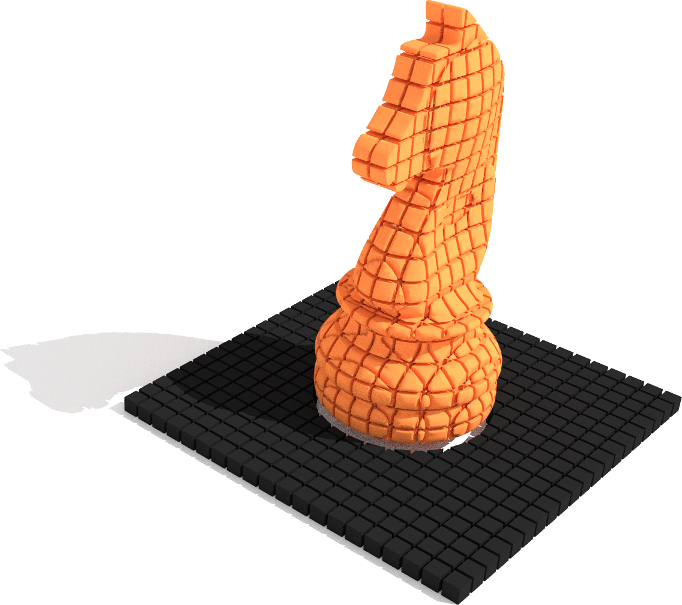
\includegraphics[width=0.35\paperwidth]{side_bar}\\
		\column{0.01\textwidth}
		\column{0.70\textwidth}
			\titlepage
			\hspace*{+0.5em}
			\begin{center}
				
\includegraphics[height=1.0cm]{lidet-logo}\\
				
\includegraphics[height=1.0cm]{ime-logo}\\
			\end{center}
	\end{columns}
	%\addtocounter{framenumber}{-1}
\end{frame}
}

% ---------------------------------------------------------------------------- %
% Other Slides (index from 1 onwards)
% ---------------------------------------------------------------------------- %

% setup navigation symbols and footline
\setbeamertemplate{navigation symbols}{}
\makeatletter
\setbeamertemplate{footline}{%
    \leavevmode%
    \hbox{%
        \begin{beamercolorbox}[wd=0.28\paperwidth,ht=4ex,dp=1ex,left,%
                               leftskip=2ex]{author in head/foot}%
            \usebeamerfont{title in head/foot}
            \insertdate\newline%
            \vskip 0.6ex%
            \autores
        \end{beamercolorbox}%
        \begin{beamercolorbox}[wd=0.53\paperwidth,ht=4ex,dp=1ex,center]%
                              {author in head/foot}%
            \usebeamerfont{author in head/foot}\lessontitle%
        \end{beamercolorbox}%
        \begin{beamercolorbox}[wd=0.19\paperwidth,ht=4ex,dp=1ex,right,%
                               rightskip=2ex]{author in head/foot}%
            \insertframenumber{}/\inserttotalframenumber \newline
            \lidet%
        \end{beamercolorbox}%
    }%
    \vskip 4cm%
}
\makeatother

% ---------------------------------------------------------------------------- %
\begin{frame}[plain]
\frametitle{\textbf{Agenda}}
	\hspace*{+4.0em}
	\footnotesize{ \tableofcontents }
\end{frame}

%* Documentação e Comunicação em Projeto (o "Game Design Document", ou GDD)
%* Caracterização do Público-Alvo (Personas)
%    - Motivação/Importância
%    - Técnicas de escrita (cartões)
%    - Além de preferências: capacidades (cognitiva e motora)
%* Mecânicas de Jogos
%    - O que é e para que serve?
%    - Relação da mecânicas com os pilares de motivação
%    - Exemplos de mecânicas básicas:
%      + Analógico:
%         . Rolar e mover
%         . Coleção de peças
%         . Alocação de entidades, etc
%      + Digital:
%         . Alocação de entidades
%         . Plataformas, alavancas, movimentos, etc
%# Atividade:
%  Elaborar mecânicas para o projeto de jogo do curso.
%  Deixar coerente com os pilares da motivação.
%  Explicitar: motivo da escolha, impacto no gameplay e relação com as personas.
%  Iniciar a construção de um GDD do projeto.

% ---------------------------------------------------------------------------- %
\section{GDD - Game Design Document}
% ---------------------------------------------------------------------------- %
% ------------------------------
\begin{frame}{\textbf{GDD - Game Design Document (Documento de Projeto do Jogo)}}
    \centering
    \begin{minipage}{7cm}
        \begin{description}
            \item[Gameplay:] ações dentro do jogo
            \vskip 1cm%
            \item[Jogabilidade:] capacidade de jogar bem
        \end{description}
    \end{minipage}
\end{frame}


% ---------------------------------------------------------------------------- %
\section{Público-alvo}
% ---------------------------------------------------------------------------- %
% ------------------------------
\begin{frame}{\textbf{Motivação e importância}}
    \centering
    \begin{minipage}{7cm}
        \begin{description}
            \item[Gameplay:] ações dentro do jogo
            \vskip 1cm%
            \item[Jogabilidade:] capacidade de jogar bem
        \end{description}
    \end{minipage}
\end{frame}

% ------------------------------
\begin{frame}{\textbf{Cartões de personas}}
    \centering
    \begin{minipage}{7cm}
        \begin{description}
            \item[Gameplay:] ações dentro do jogo
            \vskip 1cm%
            \item[Jogabilidade:] capacidade de jogar bem
        \end{description}
    \end{minipage}
\end{frame}

% ------------------------------
\begin{frame}{\textbf{Adequação às capacidades do público-alvo}}
    \centering
    \begin{minipage}{7cm}
        \begin{description}
            \item[Gameplay:] ações dentro do jogo
            \vskip 1cm%
            \item[Jogabilidade:] capacidade de jogar bem
        \end{description}
    \end{minipage}
\end{frame}


% ---------------------------------------------------------------------------- %
\section{Mecânicas de jogo}
% ---------------------------------------------------------------------------- %
% ------------------------------
\begin{frame}{\textbf{O que é mecânica de jogo?}}
    \centering
    \begin{minipage}{7cm}
        \begin{description}
            \item[Gameplay:] ações dentro do jogo
            \vskip 1cm%
            \item[Jogabilidade:] capacidade de jogar bem
        \end{description}
    \end{minipage}
\end{frame}

% ------------------------------
\begin{frame}{\textbf{Mecânicas e os pilares de motivação}}
    \centering
    \begin{minipage}{7cm}
        \begin{description}
            \item[Gameplay:] ações dentro do jogo
            \vskip 1cm%
            \item[Jogabilidade:] capacidade de jogar bem
        \end{description}
    \end{minipage}
\end{frame}


% ------------------------------
\subsection{Exemplos de mecânicas básicas}
\subsubsection{Em jogos digitais}
% ------------------------------
\begin{frame}{\textbf{}}
    \centering
    \begin{minipage}{7cm}
        \begin{itemize}
            \item Forma e função
            \vskip 1cm%
            \item Personalidade
        \end{itemize}
    \end{minipage}
\end{frame}

\subsubsection{Em jogos analógicos}
% ------------------------------
\begin{frame}{\textbf{Quadrado}}
    \centering
    \begin{figure}%
        \begin{subfigure}{0.49\textwidth}%
            \centering
            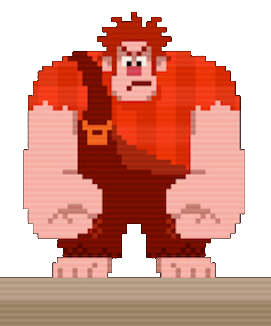
\includegraphics[height=4.5cm]{ralph}
            \caption{Ralph (Wreck it Ralph)\footnotemark{}}
        \end{subfigure}
        \begin{subfigure}{0.49\textwidth}%
            
\includegraphics[height=4.5cm]{dammd}
            \caption{Dammd (Final Fight)\footnotemark{}}
        \end{subfigure}
    \end{figure}
    \footnotetext[12]{\url{http://cache.g4tv.com/ImageDb3/303386_S/wreck-it-ralph-game-coming-from-activision-and-disney-interactive.jpg}}
    \footnotetext{\url{http://www.arcadequartermaster.com/ffight/boss_damnd.png}}
\end{frame}

\begin{frame}{\textbf{Silhueta}}
    \centering
    \begin{figure}
        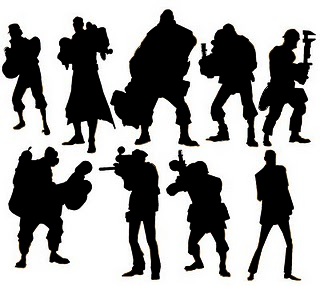
\includegraphics[height=5cm]{team_fortress2_silhueta}
        \caption{Team Fortress 2\footnote{\url{http://www.mellow3d.com/misc/tf2.png}}}
    \end{figure}
\end{frame}


% ---------------------------------------------------------------------------- %
\section{Atividade}
% ---------------------------------------------------------------------------- %

% ------------------------------
\begin{frame}{Atividade}
    \centering
    \begin{minipage}{9cm}
        \begin{itemize}
            \item Definir público alvo e montar personas
            \vskip 0.6cm%
            \item Definir (ou melhorar) as mecânicas do projeto
            \vskip 0.6cm%
            \item Mater a coerência com os pilares da motivação\\
                  \textit{(Justificar escolhas, impacto no gameplay e relação
                  com as personas)}
            \vskip 0.6cm%
            \item Elaborar GDD de página única
        \end{itemize}
	\end{minipage}
\end{frame}

\end{document}

